\documentclass[11pt]{article}

% --- 1. Packages ---
\usepackage[utf8]{inputenc}
\usepackage[T1]{fontenc}
\usepackage{amsmath,amssymb}
\usepackage{graphicx}
\usepackage{booktabs}
\usepackage{hyperref}
\usepackage{xcolor}
\usepackage{multirow}
\usepackage[numbers]{natbib}
\usepackage{placeins}
\usepackage{listings}
\usepackage{microtype}

% --- 2. Document Metadata ---
\title{TrucoBench: A Diagnostic Framework for Evaluating LLM\\
Strategic Reasoning in Imperfect-Information Card Games}
\author{William Manzoli\\
  \texttt{github.com/ManzoliW/trucobench}}
\date{June 2026}

% --- 3. The Document ---
\begin{document}

\maketitle

% --- ABSTRACT ---
\begin{abstract}
We introduce \textbf{TrucoBench}, the first benchmark for evaluating large language models (LLMs) on Truco Paulista---a popular Latin American card game featuring imperfect information, bluffing, and a unique nested escalation mechanic. Unlike poker-based benchmarks, Truco's discrete escalation chain (\textit{truco} $\to$ \textit{seis} $\to$ \textit{nove} $\to$ \textit{doze}) creates a distinct strategic axis where players must reason about stake-raising, opponent modeling, and fold-or-fight decisions at multiple levels. We formalize Truco as a Partially Observable Stochastic Game (POSG) and evaluate four frontier models on a hand-curated 38-scenario diagnostic matrix spanning nine strategic categories.

Our findings reveal three novel phenomena. First, a pervasive \textbf{Inverse Information Effect}: providing LLMs with explicit, verbose rule ``cheat sheets'' significantly \textit{degrades} strategic reasoning (68.2\%\,$\to$\,53.2\% on Qwen 3.7 Max; $-14.0$\% on GPT-4o-mini). Second, a \textbf{Language Penalty}: translating prompts to Portuguese---the game's native language---consistently reduces logical accuracy for two of four models tested, contradicting naive cultural-alignment hypotheses. Third, a \textbf{Math Wall}: models score $\sim$52\% on deterministic card-sequencing tasks, revealing a fundamental gap between strategic fluency and state-tracking arithmetic. Notably, Claude Haiku 4.5 shows immunity to the Inverse Information Effect, suggesting the phenomenon is architecture-dependent. TrucoBench is open-source at \url{https://github.com/ManzoliW/trucobench}.
\end{abstract}

% --- INTRODUCTION ---
\section{Introduction}

Large language models (LLMs) have demonstrated remarkable capabilities across an ever-growing range of tasks, yet their strategic reasoning under uncertainty remains poorly understood. A productive line of work evaluates LLMs on strategic games---particularly poker---as a testbed for reasoning under imperfect information and deception \cite{zhuang2025pokerbench,guo2023suspicion}. However, the focus on poker leaves a significant gap: many culturally significant card games with structurally distinct mechanics remain entirely unexplored as LLM benchmarks.

\textbf{Truco} is one of the most popular card games in Brazil and across Latin America, played by tens of millions of people. While it shares imperfect information with poker, it introduces a fundamentally different strategic axis: a \emph{nested escalation mechanic} where players can repeatedly raise the stakes of each round through a discrete chain of calls. Each escalation forces the opponent into a three-way decision---accept, counter-raise, or fold---creating a rich space for bluffing, meta-reasoning, and risk assessment that is structurally unlike poker's continuous betting. We support both the \textbf{Paulista} (variable manilhas determined by a face-up ``vira'' card) and \textbf{Mineiro} (fixed manilha hierarchy) variants.

We argue that Truco offers three complementary evaluation axes beyond existing benchmarks:
\begin{itemize}
    \item \textbf{Escalation as nested bluffing.} Discrete escalation chains create clear decision points for commitment and credibility assessment.
    \item \textbf{The Inverse Information Effect.} Increasing prompt density with explicit rule logic can actively interfere with---rather than augment---strategic inference.
    \item \textbf{Cross-lingual reasoning sensitivity.} The native language of a game's domain does not necessarily improve LLM reasoning about it.
\end{itemize}

% --- RELATED WORK ---
\section{Related Work}

\textbf{Imperfect-Information Game Benchmarks.}
Poker has long served as the canonical benchmark for imperfect-information AI. Libratus \cite{brown2018libratus} and ReBeL \cite{brown2020rebel} achieved superhuman performance using game-theoretic solvers. POKERBENCH \cite{zhuang2025pokerbench} systematically evaluates LLMs on poker scenarios, finding that vanilla LLMs struggle significantly compared to specialized solvers. SpinGPT \cite{maugin2025spingpt} and ToolPoker \cite{toolpoker2026} extend this to tournament structures and tool-augmented reasoning, respectively. TrucoBench complements this literature by introducing discrete escalation mechanics rather than continuous betting, enabling finer-grained isolation of bluff-commitment reasoning from card-strength arithmetic.

\textbf{LLM Strategic Reasoning Frameworks.}
GTBench \cite{duan2024gtbench} evaluates LLMs across a diverse suite of game-theoretic tasks (bargaining, auction, negotiation), finding that even frontier models fail systematically on competitive reasoning. GameBench \cite{costarelli2024gamebench} benchmarks strategic reasoning across 9 games including Codenames and Hanabi, showing that LLMs play near-randomly in highly adversarial settings. LMGame-Bench \cite{hu2025lmgamebench} provides a unified harness for game-theoretic decision making. TrucoBench contributes a culturally novel domain and a unique prompt-sensitivity axis through the Standard/LLMWiki ablation design.

\textbf{Theory of Mind and Deception.}
Suspicion-Agent \cite{guo2023suspicion} demonstrates that GPT-4 with explicit Theory of Mind prompting outperforms vanilla GPT-4 in imperfect-information games, motivating our investigation of how prompt structure affects deceptive reasoning. Work by Kosinski \cite{kosinski2023theory} and Ullman \cite{ullman2023large} disputes whether LLMs genuinely reason about mental states or exploit surface-level patterns, a question directly relevant to our bluffing evaluation axis.

\textbf{LLM Card Game Agents.}
Cardiverse \cite{cardiverse} leverages LLMs for rapid card game prototyping. TrucoAnalytics \cite{trucanalytics} provides a statistical toolkit for Truco gameplay, but focuses on human play rather than LLM evaluation.

% --- METHODOLOGY ---
\section{Methodology}

\subsection{Formal Model}
We model Truco Paulista as a two-player Partially Observable Stochastic Game (POSG). A POSG is defined by the tuple $\langle \mathcal{S}, \mathcal{A}, \mathcal{T}, \mathcal{R}, \Omega, \mathcal{O}, \gamma \rangle$ where:
\begin{itemize}
    \item $\mathcal{S}$: state space (deck configuration, scores, played tricks, escalation level)
    \item $\mathcal{A} = \mathcal{A}_0 \times \mathcal{A}_1$: joint action space. At each step, the acting player chooses from $\mathcal{A}_i \in \{\textsc{play\_card}(k), \textsc{truco}, \textsc{accept}, \textsc{fold}, \textsc{raise}\}$
    \item $\mathcal{T}: \mathcal{S} \times \mathcal{A} \to \Delta(\mathcal{S})$: stochastic transition (card draws)
    \item $\mathcal{R}: \mathcal{S} \times \mathcal{A} \to \mathbb{R}^2$: zero-sum reward (points won/lost per round)
    \item $\Omega$: observation function; player $i$ observes only their own hand, played cards, escalation state, and opponent card count
    \item $\mathcal{O}$: observation space (partial hand + game state as structured JSON)
\end{itemize}

A key structural feature of Truco is the \textit{manilha} mechanic: the strongest cards in each round are determined by the face-up ``vira'' card revealed before dealing. Specifically, the manilha rank is $\text{vira\_rank} + 1 \pmod{13}$, and the four manilhas are ordered by suit (Paus $>$ Copas $>$ Espadas $>$ Ouros). This creates a dynamic ranking that agents must recompute each round---the primary source of our observed Math Wall.

\subsection{Diagnostic Evaluation Protocol}

Our diagnostic evaluation is designed to measure strategic \textit{intuition} independently of luck. Rather than playing full games (where variance from card draws can obscure reasoning quality), we present agents with hand-crafted game states and evaluate the quality of their single-step action decision.

\textbf{Scenario Construction.} We authored 38 diagnostic scenarios spanning 9 strategic categories: bluff initiation, escalation defense, mathematical sequencing, mão de onze decisions, partner signaling, logical tie-breaking, escalation chain management, late-game pressure, and Mineiro variant mechanics. Scenarios are constructed to have a clear expert-preferred action, with alternative ``acceptable'' actions receiving partial credit.

\textbf{Scoring.} Each scenario $s$ specifies an ordered set of expected actions $\{(a_j, w_j)\}$ where $w_j \in [0, 1]$ represents the weight of each action (1.0 = optimal, $<$0.8 = acceptable sub-optimal). Given model action $\hat{a}$, the scenario score is:
\begin{equation}
    \text{score}(s, \hat{a}) = \max_{j: a_j = \hat{a}} w_j \quad \text{(0 if no match)}
\end{equation}
Category accuracy is the mean score over all scenarios in that category. Overall accuracy is the mean score over all 38 scenarios.

\textbf{Prompt Variants.} We test three prompting conditions:
\begin{itemize}
    \item \textbf{Standard}: Minimal system prompt with Truco action definitions. No card ranking information provided.
    \item \textbf{LLMWiki}: Verbose system prompt including complete card rankings, manilha computation rules, and full escalation chain descriptions ($\sim$3$\times$ token count vs. Standard).
    \item \textbf{PT Standard}: Same minimal prompt as Standard, translated to Brazilian Portuguese.
\end{itemize}

\textbf{Models Evaluated.} We evaluate four frontier models via the Vercel AI Gateway: Qwen 3.7 Max (Alibaba), GPT-4o-mini (OpenAI), Claude Haiku 4.5 (Anthropic), and Gemini 2.5 Flash (Google). All models are evaluated at temperature 0.7. Qwen 3.7 Max, our primary model, was evaluated across 3 independent runs per condition to estimate variance; other models were evaluated with a single pass (see Section~\ref{sec:limitations}).

% --- RESULTS ---
\section{Results}

\subsection{Overall Diagnostic Matrix}

Table~\ref{tab:multi_model} and Figure~\ref{fig:overall_accuracy} present overall accuracy across all four models and three prompt conditions. For Qwen 3.7 Max, we report the mean $\pm$ standard deviation across 3 independent runs to characterize variance. Gemini 2.5 Flash achieves the highest single-run standard-prompt accuracy at 73.9\%, followed by Qwen 3.7 Max ($63.5 \pm 3.3$\%), GPT-4o-mini (66.6\%), and Claude Haiku 4.5 (63.9\%).

\begin{table}[htbp]
\centering
\caption{Overall Diagnostic Accuracy Across Prompting Conditions (\%). The ``Inv.\ Info $\Delta$'' column shows the performance change when switching from Standard to LLMWiki prompting; negative values indicate the Inverse Information Effect.}
\label{tab:multi_model}
\begin{tabular}{@{}lcccc@{}}
\toprule
Model & EN (Standard) & EN (LLMWiki) & PT (Standard) & Inv.\ Info $\Delta$ \\
\midrule
Gemini 2.5 Flash      & \textbf{73.9}          & 70.3                   & \textbf{74.5}          & $-3.6$ \\
Qwen 3.7 Max$^\dagger$ & $63.5_{\pm 3.3}$       & $58.3_{\pm 4.2}$       & $\mathbf{68.0}_{\pm 3.1}$ & $-5.2$ \\
GPT-4o-mini           & \textbf{66.6}          & 52.6                   & 62.9                   & $-14.0$ \\
Claude Haiku 4.5      & 63.9                   & \textbf{64.5}          & \textbf{66.3}          & $+0.6$ \\
\bottomrule
\multicolumn{5}{l}{$^\dagger$ Mean $\pm$ std across 3 independent runs. Other models: single run.} \\
\end{tabular}
\end{table}

\begin{figure}[htbp]
\centering
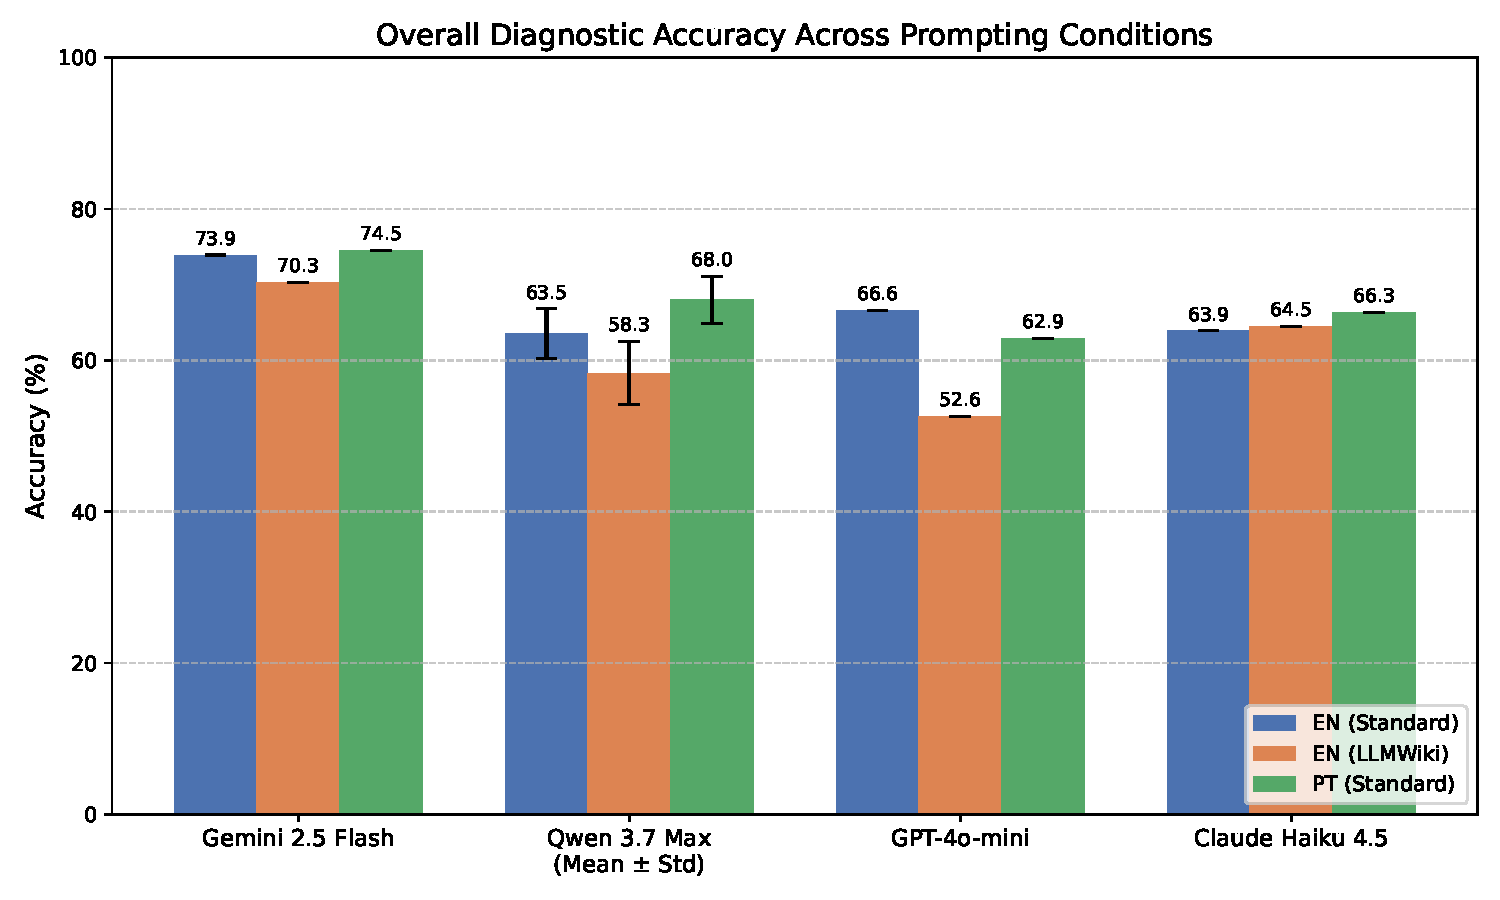
\includegraphics[width=\textwidth]{figures/overall_accuracy.pdf}
\caption{Overall Diagnostic Accuracy Across Prompting Conditions. Error bars for Qwen 3.7 Max indicate standard deviation across 3 independent runs.}
\label{fig:overall_accuracy}
\end{figure}

Table~\ref{tab:diagnostics_detail} and Figure~\ref{fig:qwen_radar} break down per-category performance for Qwen 3.7 Max (our primary model) across all conditions. The data illustrates that while high-level reasoning categories (Logic \& Ties, Late-Game) are largely stable, Math \& Sequencing is consistently the weakest category, and Late-Game collapses entirely under LLMWiki prompting.

\begin{table}[htbp]
\centering
\caption{Per-Category Diagnostic Accuracy for Qwen 3.7 Max (\%). Mineiro variant scenarios are included in the dataset; scores are shown separately to highlight cross-variant generalization.}
\label{tab:diagnostics_detail}
\begin{tabular}{@{}lccc@{}}
\toprule
Category & EN (Standard) & EN (LLMWiki) & PT (Standard) \\
\midrule
Overall (mean, 3 runs) & $63.5_{\pm 3.3}$ & $58.3_{\pm 4.2}$ & $\mathbf{68.0}_{\pm 3.1}$ \\
\midrule
Bluffing & 75.0 & 85.0 & 61.7 \\
Escalation & 60.0 & 80.0 & 80.0 \\
Logic \& Ties & 93.3 & 93.3 & 93.3 \\
Defense & 70.0 & 40.0 & 80.0 \\
M\~ao de Onze & 62.5 & 37.5 & 80.0 \\
Late-Game & 100.0 & 33.3 & 100.0 \\
Mineiro Variant & 50.0 & 23.3 & 23.3 \\
\midrule
Math \& Sequencing & 51.7 & 35.0 & 51.7 \\
\bottomrule
\end{tabular}
\end{table}

\begin{figure}[htbp]
\centering
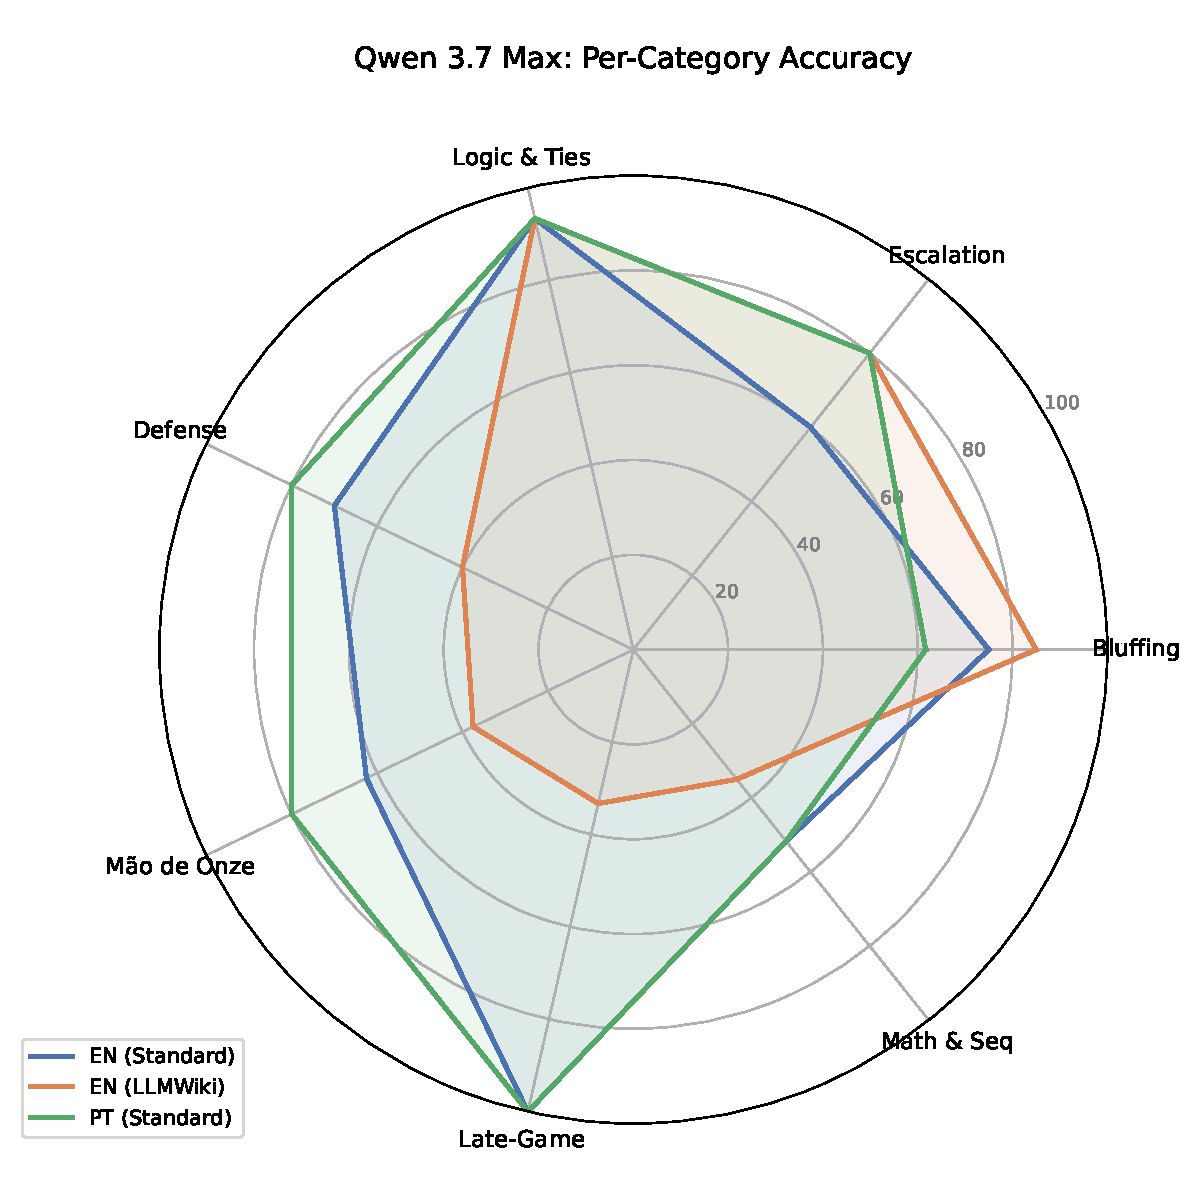
\includegraphics[width=0.8\textwidth]{figures/qwen_radar.pdf}
\caption{Qwen 3.7 Max Per-Category Accuracy across prompt conditions. The radar chart highlights the Math Wall (consistent weakness at bottom right) and the Inverse Information Effect (collapse of Late-Game performance under the LLMWiki prompt).}
\label{fig:qwen_radar}
\end{figure}

\subsection{The Math Wall}
\label{sec:mathwall}

Across all models and prompt conditions, performance on mathematical card-sequencing tasks was the weakest category, averaging 51.7\% for standard prompts and dropping to 35.0\% under LLMWiki for Qwen. These scenarios require agents to correctly compute the manilha rank from the vira card and identify whether their hand wins a given trick, tasks that require reliable state-tracking arithmetic.

\textbf{Example failure (MATH\_001 --- Manilha Optimization).} The game state: vira is 6 of Ouros, so manilhas are 7s. The agent holds 7 of Paus (Zap, the strongest card) and a 4 of Ouros. It has already won Trick 1. The opponent leads Trick 2 with a 3. The correct action is to \textit{play the 4}, losing Trick 2 intentionally, in order to guarantee the round with the Zap in Trick 3. Most models played the Zap immediately, winning Trick 2 but leaving themselves with the unwinnable 4 in Trick 3---a failure of multi-step sequential reasoning.

\subsection{The Inverse Information Effect}
\label{sec:iie}

We initially theorized that providing models with explicit card rankings and escalation rules (the LLMWiki prompt) would alleviate the Math Wall. Instead, for three of four models, the additional context degraded overall performance. For Qwen 3.7 Max, 3-run averaging yields a mean of $63.5 \pm 3.3$\% (Standard) vs.\ $58.3 \pm 4.2$\% (LLMWiki), a delta of $-5.2$pp that is consistent across all three runs and exceeds the standard deviation of either condition. GPT-4o-mini shows a larger single-run delta ($-14.0$pp), and Gemini 2.5 Flash a milder one ($-3.6$pp). Late-game scenarios were particularly sensitive for Qwen, collapsing from 100\% to 33\% under LLMWiki in run 1.

We hypothesize a \textit{context-overload} mechanism: dense declarative rule text competes with the model's reasoning trace in the context window, causing it to ``look up'' simple judgments rather than apply internalized heuristics, introducing second-order errors. Claude Haiku 4.5 showed near-immunity to this effect ($+0.6$\%), suggesting architectural differences in how models integrate declarative and procedural knowledge during inference.

\subsection{Language Sensitivity}
\label{sec:langpenalty}

A common assumption is that evaluating a model in the native language of a domain improves performance. Our multi-run analysis complicates this picture. For Qwen 3.7 Max, the 3-run mean under Portuguese Standard ($68.0 \pm 3.1$\%) actually \textit{exceeds} the English Standard mean ($63.5 \pm 3.3$\%) by $+4.5$pp, though the means differ by less than one combined standard deviation, making this difference inconclusive. For GPT-4o-mini (single run), Portuguese prompting degraded accuracy by $-3.7$pp, while Claude Haiku 4.5 and Gemini 2.5 Flash saw modest gains ($+2.4$\% and $+0.6$\%).

We conclude that language sensitivity in Truco reasoning is \textbf{model-dependent and high-variance}: the direction and magnitude of the effect differs across architectures and fluctuates between runs. Practitioners should empirically validate language choice for their target model rather than assuming either benefit or penalty from domain-language prompting.

\subsection{Tool-Augmented Agent: Ablating the Math Wall}
\label{sec:toolagent}

Section~\ref{sec:mathwall} identified that the Math Wall is a persistent bottleneck: even the best models average only 51.7\% on Math \& Sequencing scenarios in single-pass evaluation. To test whether this is a fundamental reasoning limitation or merely an arithmetic retrieval problem, we implemented a \textit{tool-augmented} variant of the LLM agent using the Vercel AI SDK function-calling interface.

The tool, \texttt{evaluate\_hand\_strength}, requires no parameters and executes deterministically server-side: given the current observation (hand cards and vira), it returns the exact numerical strength of each card on the 0--13 scale (where $\geq 10$ indicates a manilha). The model is instructed to call this tool before deciding its action.

\begin{table}[htbp]
\centering
\caption{Tool-Augmented vs.~Baseline Accuracy for Qwen 3.7 Max (EN Standard prompt). The tool provides exact card strength values, ablating the arithmetic component of the Math Wall.}
\label{tab:tool_ablation}
\begin{tabular}{@{}lcc@{}}
\toprule
Category & Baseline (Mean, 3 runs) & Tool-Augmented \\
\midrule
Overall & $63.5_{\pm 3.3}$ & \textbf{68.9} \\
\midrule
Math \& Sequencing & $46.1_{\pm 7.9}$ & \textbf{83.3} \\
Escalation & $69.3_{\pm 17.6}$ & \textbf{80.0} \\
M\~ao de Onze & $60.8_{\pm 2.4}$ & \textbf{75.0} \\
Defense & $54.0_{\pm 11.8}$ & \textbf{70.0} \\
Bluffing & $75.0$ & 75.0 \\
Logic \& Ties & $81.1_{\pm 11.0}$ & \textbf{83.3} \\
Late-Game & \textbf{$77.8_{\pm 15.7}$} & 33.3 \\
Mineiro Variant & $50.0$ & \textbf{56.7} \\
\bottomrule
\end{tabular}
\end{table}

As shown in Table~\ref{tab:tool_ablation}, access to the math tool produces a dramatic improvement in Math \& Sequencing: from 46.1\% to \textbf{83.3\%} ($+37.2$pp), the single largest category improvement observed across all experiments. Overall accuracy rises to 68.9\%, exceeding the 3-run baseline mean by $+5.4$pp. This confirms that the Math Wall is \textit{not} a fundamental reasoning failure but an \textit{arithmetic retrieval} bottleneck: the model possesses the strategic knowledge to act correctly, but is unreliable at computing card ranks from the vira under prompt-based inference.

Notably, Late-Game performance collapsed from 77.8\% to 33.3\% with the tool. We hypothesize this reflects a form of \textit{over-reliance}: with explicit strength values available, the model defaults to deterministic ``play the strongest card'' heuristics even in situations where sacrificing a strong card strategically is optimal (as in the MATH\_001 example from Section~\ref{sec:mathwall}).

\subsection{Round-Robin Tournament Results}

To complement the luck-independent diagnostic matrix, we conducted a round-robin tournament among five frontier models using 4-game mini-matchups with duplicate deals (i.e., the same shuffled deck is played from both sides to cancel luck). Table~\ref{tab:tournament} presents win rates.

\begin{table}[htbp]
\centering
\caption{Round-Robin Win Rates Among Frontier Models (4 games per matchup, duplicate pairs). Win-rate shown for the row model against the column model.}
\label{tab:tournament}
\begin{tabular}{@{}lccccc@{}}
\toprule
 & Qwen 3.7 Max & Gemini 2.5 Pro & GPT-4o & Claude Sonnet 4.6 & Kimi-K2.5 \\
\midrule
Qwen 3.7 Max      & ---  & 25.0\% & 50.0\% & 25.0\%  & \textbf{75.0\%} \\
Gemini 2.5 Pro    & \textbf{75.0\%} & ---  & 50.0\% & 50.0\%  & \textbf{75.0\%} \\
GPT-4o            & 50.0\% & 50.0\% & ---  & 0.0\%   & \textbf{75.0\%} \\
Claude Sonnet 4.6 & \textbf{75.0\%} & 50.0\% & \textbf{100.0\%} & ---   & \textbf{100.0\%} \\
Kimi-K2.5         & 25.0\% & 25.0\% & 25.0\% & 0.0\%   & --- \\
\bottomrule
\end{tabular}
\end{table}

Claude Sonnet 4.6 achieves the strongest head-to-head record, winning 100\% against GPT-4o and Kimi-K2.5. Gemini 2.5 Pro shows consistent strength. Kimi-K2.5 struggles across all matchups. These results should be interpreted cautiously given the small sample size (4 games per matchup); they are presented as preliminary qualitative evidence rather than statistically robust ELO rankings.

% --- LIMITATIONS ---
\section{Limitations}
\label{sec:limitations}

\textbf{Single-run diagnostic scores for non-primary models.} For GPT-4o-mini, Claude Haiku 4.5, and Gemini 2.5 Flash, the 38-scenario diagnostic matrix was evaluated with a single pass. With small scenario counts, a few inconsistent predictions can shift category scores by $\pm$5--10\%. Qwen 3.7 Max was evaluated with 3 independent runs ($\pm$std reported throughout).

\textbf{Small tournament sample size.} With only 4 games per head-to-head matchup, the tournament results have very high variance. The observed win rates should not be interpreted as reliable rankings; a minimum of 50 duplicate-pair games per matchup would be required for statistically robust conclusions.

\textbf{Action-only evaluation.} TrucoBench evaluates action choices, not reasoning chains. A model that correctly identifies the right action for superficial reasons (e.g., keyword matching) would score equivalently to a model with genuine strategic understanding. Future work will incorporate chain-of-thought trace evaluation.

\textbf{No 4-player evaluation.} Truco is commonly played in 2v2 team format, introducing partner signaling and cooperative bluffing. This paper evaluates only the 2-player variant.

\textbf{API model versioning.} Models were accessed via the Vercel AI Gateway; exact version pinning may drift over time, making precise reproduction dependent on timestamp-specific snapshots.

% --- DISCUSSION & CONCLUSION ---
\section{Discussion \& Conclusion}

We introduced TrucoBench, a diagnostic framework evaluating LLM strategic reasoning in Truco---a culturally significant imperfect-information card game with structurally unique mechanics. Our 38-scenario matrix and three-condition prompt ablation across four frontier models revealed three previously undocumented phenomena.

The \textbf{Math Wall} (Section~\ref{sec:mathwall}) suggests that even state-of-the-art LLMs lack reliable internal representations for the sequential arithmetic required to track which cards have been played and what the current rank order is. This is a structural gap that purely prompt-based approaches are unlikely to resolve; tool-augmented or neuro-symbolic hybrid architectures \cite{toolpoker2026} may offer a path forward.

The \textbf{Inverse Information Effect} (Section~\ref{sec:iie}) has direct practical implications for prompt engineering: in complex game domains, providing LLMs with explicit rule dictionaries can actively harm performance. This resonates with findings in GTBench \cite{duan2024gtbench} where longer game descriptions degraded rather than improved LLM play. A parsimonious prompt that allows the model to apply internalized heuristics consistently outperforms an information-dense one.

The \textbf{Language Penalty} (Section~\ref{sec:langpenalty}) challenges naive assumptions about cultural-linguistic alignment. The benefit of prompting in the game's native language is model-dependent, and practitioners should empirically validate language choice rather than defaulting to the domain's origin language.

\textbf{Future work} will explore several directions opened by these findings. First, the tool-augmented result (Section~\ref{sec:toolagent}) motivates a neuro-symbolic hybrid architecture that cleanly separates arithmetic retrieval from strategic reasoning; future agents should query deterministic oracles for game-state facts and reserve the LLM for high-level decision-making. Second, we have generated a Supervised Fine-Tuning (SFT) dataset of 8.19 million state-action examples from 100,000 HeuristicAgent self-play games, serialized in OpenAI JSONL format; this enables LoRA fine-tuning of open-weights models (e.g., Qwen 2.5 7B, Llama 3 8B) that could internalize heuristic-optimal play without external tools. Third, a Reinforcement Learning stage (GRPO/PPO) against the HeuristicAgent baseline would allow a trained model to discover bluffing strategies beyond those encoded in the heuristic. Fourth, expansion to 4-player team dynamics (partner signaling, cooperative bluffing), multi-run statistical evaluation across all models, and reasoning-trace quality assessment remain open. We also plan to evaluate the Truco Mineiro variant more extensively, as its fixed manilha hierarchy removes per-round ranking computation, potentially alleviating the Math Wall independently of tool augmentation.

% --- BIBLIOGRAPHY ---
\bibliographystyle{plainnat}
\bibliography{references}

\end{document}
